\documentclass[10pt]{article}

\usepackage{polski}
\usepackage{graphicx}
\usepackage{hyperref}
\graphicspath{{images/}}

\usepackage{geometry}
\newgeometry{tmargin=4cm, bmargin=4cm, lmargin=3.2cm, rmargin=3.2cm}

\usepackage{fancyhdr}
\pagestyle{fancy}



\begin{document}

\begin{titlepage}


\begin{center}

  \LARGE \textsc{Politechnika Wrocławska}\\
  \vspace*{0.2cm}
  \Large \textsc{Wydział Informatyki i Telekomunikacji}\\
  \vspace*{0.4cm}
  \centering
\includegraphics[width=0.2\textwidth]{WITlogo.png}\\
  \vspace*{0.2cm}
  \vspace*{2cm}

  \centerline{\rule{\textwidth}{1.2pt}}
  \vspace{0.4cm}
  \Huge\textbf{Metody i Systemy Decyzyjne}
  \centerline{\rule{\textwidth}{1.2pt}}
  \vspace{1cm}
  \LARGE Sprawozdanie z laboratorium\\
  \vspace{3.5cm}
  \textsc{Autor}\\
  \vspace{0.2cm}
  \textbf{Krzysztof Szuba}\\
  \vspace{0.1cm}
  \Large nr albumu: \textbf{260298}\\
  \vspace{0.1cm}
  kierunek: \textbf{Informatyka Stosowana}

  \vspace*{\fill}
  \Large \textit{\today}

 \end{center}


\end{titlepage}


\begin{abstract}
Celem pracy jest przeanalizowanie pandemii COVID-19 od 24.02.2020 do 06.03.2022 roku. Głównie skupiłem się na zbadniu zależności między zamożnością i gęstością zaludnienia państw a rozwojem epidemii. W notebook'u przedstawiłem wiele wizualizacji, tutaj opiszę tylko wspomniany problem. 
\end{abstract}

\section{Wstęp -- sformułowanie problemu}
\label{sec:wstep}
W ciągu ostatnich 2 lat nasze życie stanęło do góry nogami. COVID-19 rozprzestrzenił się na wszystkich zamieszkałych kontynentach. Jakie są główne czynniki sytuacji epidemicznej w krajach? Czy jest to ich zamożność, czy może gęstość zaludnienia? W teorii, wirus w najgęściej zaludnionych panśtwach powinien rozwijać się na większą skalę. Bogatsze kraje dużo lepiej powinny sobie radzić z zaistniałą sytuacją. W tym miejscu wyjaśnie również dwa niezbędne, badane terminy.

\begin{itemize}
    \item \textbf{Zachorowalność}(ang. Incidence rate) - jako współczynnik zachorowalności przyjąłem całkowitą liczbę przypadków zarażenia wirusem podzieloną przez liczbę mieszkańców w danym regionie
    \item \textbf{Śmiertelność}(ang. Death rate) - jako współczynnik śmiertelności przyjąłem całkowitą liczbę zgonów podzieloną przez liczbę zakażeń
\end{itemize}

\section{Opis rozwiązania} 
 Dane pobrałem ze strony \url{https://covid.ourworldindata.org/data/owid-covid-data.csv}. Korzystając z biblioteki Pandas utworzyłem ramkę danych. Każdy rekord zawierał informacje o każdym dniu pandemii dla każdego regionu na świecie. Mnie interesowały ogólne statystki, więc musiałem odpowiednio oczyścić i przygotować dane. Wizualizacje danych zrobiłem głownię za pomocą biblioteki Plotly. Wykresy dla sformułowanych problemów za pomocą Matplotlib. Dzięki sklearn stworzyłem modele liniowe. 

\section{Rezultaty obliczeń}

\subsection{Plan badań}
Na początku - żeby się upewnić, że zamożność państw ma jakikolwiek wpływ na koronawirusa, stworzyłem dwa diagramy słupkowe. Przedstawiały one zachorowalność oraz śmiertelność dla państw podzielonych na podstawie ich bogactwa. 

\begin{center}
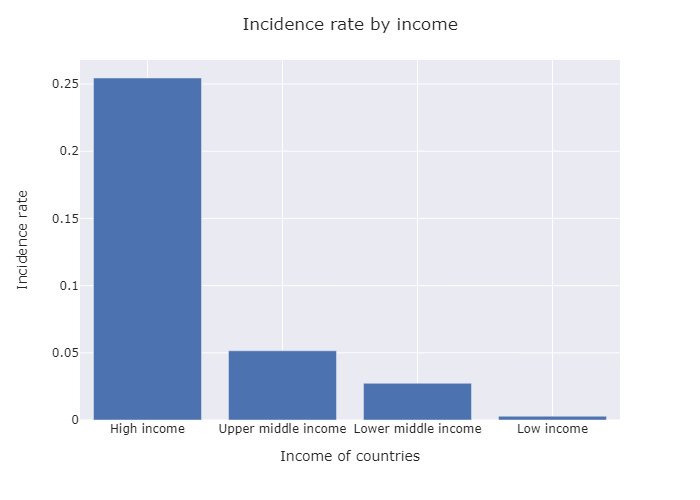
\includegraphics[width=0.8\linewidth]{incidence_rate_income.png}
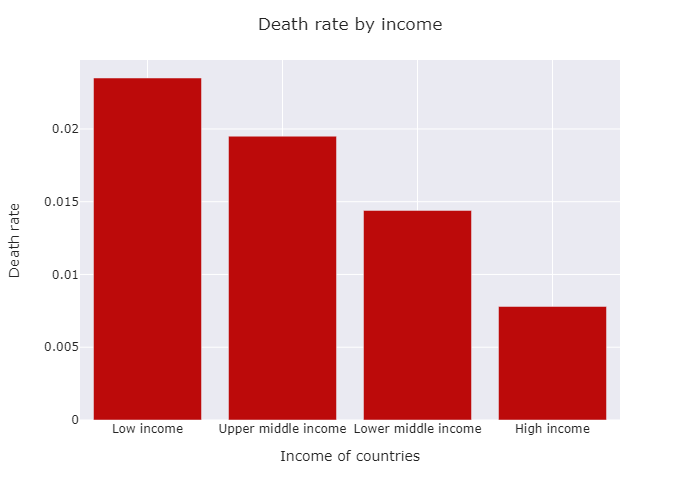
\includegraphics[width=0.8\linewidth]{death_rate_income.png}
\end{center}
Jak widać zamożność państw ma wpływ na rozwój choroby. Bogatsze państwa zmagają się z większą zachorowalnością, a biedniejsze mają wyższą śmiertelność. Wiedząc to, mogłem przystąpić do badania zaleznośći między PKB na osobę a tymi współczynnikami.

\subsection{Wyniki obliczeń}
\subsubsection{Zależność zachorowalności od gęstości zaludnienia}
\begin{center}
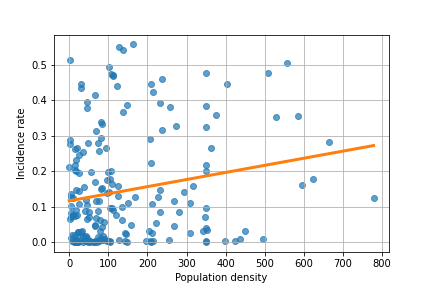
\includegraphics[width=0.8\linewidth]{incidence_density.png}
\end{center}
Na powyższym wykresie wyraźnie widać brak zależności liniowiej między zmiennymi. 
Również współczynnik korelacji wynoszący 0,195 wskazuje na brak zależności.
\textbf{Regresją liniową nie można przewidzieć zachorowalności na podstawie gęstości zaludnienia.}
\subsubsection{Zależność zachorowalności od PKB na mieszkańca}
\begin{center}
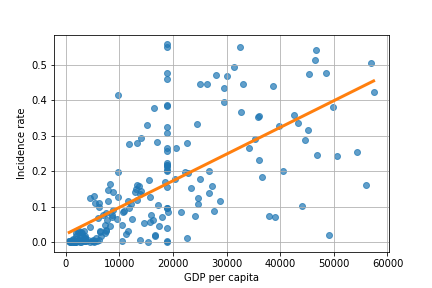
\includegraphics[width=0.8\linewidth]{gdp_incidence.png}
\end{center}
Współczynnik korelacji wynosi prawie 0,7 co wskazuje na dość silny związek korelacyjny. 
Mimo to widać brak zależności liniowej między zmiennymi, \textbf{co wyklucza regresję liniową jako dobrą metodę do przewidywania zachorowalności na podstawie PKB na mieszkańca.}
\newpage
\subsubsection{Zależność śmiertelności od PKB na mieszkańca}
\begin{center}
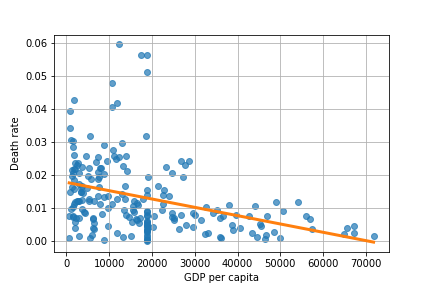
\includegraphics[width=0.8\linewidth]{death_gdp.png}
\end{center}
Współczynnik korelacji to -0,36 i oznacza słaby związek korelacyjny. Tak samo jak w poprzednich przypadkach - nie widać tu zależności liniowej, więc \textbf{nie można przewidzieć współczynnika śmiertelności za pomocą regresji liniowej.}

\section{Wnioski}
Na podstawie analizy powyższych zależności można wysnuć dwa wnioski. 
\newline \textbf{Gęstość zaludnienia} państwa nie ma wpływu na jego sytuację epmidemiczną.
Wydawałoby się, że jest na odwrót. I pewnie tak jest - ale w skali miast. Czynnik ten jest po prostu bardzo względny. Ludność w lepiej zurbanizowanych krajach ma tendencję do zamieszkiwania w dużych aglomeracjach miejskich. Społeczeństwo w tych najmniej zurbanizowanych(np. Afryka) jest rozsiana po całym kraju. Weźmy na przykład Rosję. Ogromne państwo, jednak ludność jest skoncentrowana głównie w Moskwie czy Petersburgu. Gęstość zaludnienia w skali kraju nie ma znaczenia skoro znacząca wiekszość społeczeństwa zamieszkuje miasta. 
\newline \textbf{PKB na mieszkańca} ma duży wpływ na sytuację epidemiczną w kraju.
Bogate państwa mają znacznie większy współczynnik zachorowalności niż biedne. Ludzie dużo więcej podróżują czy korzystają z komunikacji miejskiej. Wirus "lepiej" rozprzestrzenia się w dużych aglomeracjach miejskich, które są cechą bogatych krajów. Śmiertelność jest jednak wyższa w biednych regionach. Zamożniejsze państwa mają dużo lepszą opiekę zdrowotną, mimo że borykają się ze znacznie większą ilością ludzi zarażonych.

\end{document}
